\chapter{ Μετρικές}
\label{chap:6}

\section{Αξιολόγηση κατά την Εκπαίδευση}
\label{sec:6.1}

Κατά τη διάρκεια της εκπαίδευσης έγινε χρήση δύο μετρικών, της Binary Cross-Entropy loss και της Ακρίβειας(Αccuracy). Οι 2 παραπάνω μετρικές χρησιμοποιήθηκαν για την αξιολόγηση του μοντέλου κατά τη διάρκεια της εκπαίδευσης για το σύνολο εκπαίδευσης και το σύνολο επικύρωσης. 

\subsection{Binary Cross-Entropy loss}
\label{subsec:6.1.1}
H Binary Cross-Entropy loss είναι μία συνάρτηση που χρησιμοποιείται σε δυαδικά προβλήματα και μετράει την επίδοση ενός μοντέλου ταξινόμησης του οποίου η έξοδος είναι μία πιθανότητα στο διάστημα [0,1]. Η μετρική αυξάνεται όσο η προβλεπόμενη 
πιθανότητα αποκλίνει από την πραγματική κλάση που ανήκει. Για ένα μοντέλο που πάντα προβλέπει σωστά, η τιμή της μετρικής θα είναι $0$. Για κάποιο δεδομένο εισόδου η μετρική ορίζεται από την εξίσωση:

\begin{equation}
loss = -ylog(p) - (1-y) log(1 -p)
\end{equation}

όπου y η πραγματική κλάση του δεδομένου εισόδου με τιμή $0$ ή $1$ και p η πιθανότητα που προέβλεψε το μοντέλο. Αν για παράδειγμα μία είσοδος άνηκε στην κλάση $0$ και η πρόβλεψη του μοντέλου ήταν $0.1$, τότε το σφάλμα θα ήταν 0.045. Αντίθετα αν η πρόβλεψη ήταν $0.4$, τότε το σφάλμα θα ήταν $0.22$, δηλαδή πολύ μεγαλύτερο. Στην εικόνα \ref{figure:cross} παρουσιάζεται η συνάρτηση Binary Cross-Entropy loss για εισόδους με πραγματική τιμή $1$. Όταν η πρόβλεψη του μοντέλου είναι κοντά στο $1$ το σφάλμα μηδενίζεται, αντίθετα για προβλέψεις κοντά στο $0$ το σφάλμα απειρίζεται. Να σημειωθεί ότι η μετρική για όλα τα δεδομένα υπολογίζεται ως ένας μέσος όρος όλων των σφαλμάτων των δεδομένων. Κατά την διάρκεια της εκπαίδευσης η συγκεκριμένη μετρική χρησιμοποιήθηκε ως ένα εποπτικό μέσο για την επίδοση του μοντέλου. Στο τέλος κάθε εποχής υπολογίζονταν το σφάλμα  για το σύνολο εκπαίδευσης και το σύνολο επικύρωσης. Επιπλέον, το μοντέλο με το μικρότερο σφάλμα Binary Cross-Entropy για τα δεδομένα επικύρωσης σε μία εποχή, αποθηκεύονταν ως το τελικό μοντέλο του πειράματος. 

\begin{figure}[!h]
    \centering
      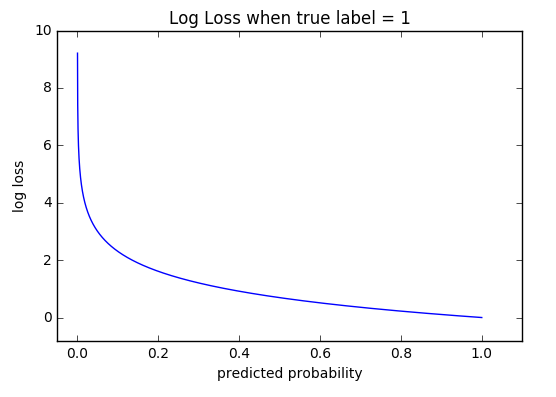
\includegraphics[width=0.6\linewidth]{crossentropy.png} \caption{Συνάρτηση Binary Cross-Entropy loss για δεδομένα της κλάσης 1}
\label{figure:cross}    
\end{figure}
  
  
\subsection{Ακρίβεια(Accuracy)}
\label{subsec:6.1.2}
Η ακρίβεια ορίζεται από τον τύπο \ref{eq:acc}. Κατά την διάρκεια της εκπαίδευσης χρησιμοποιήθηκε ως ένα εποπτικό μέσο για την επίδοση του μοντέλου. Στο τέλος κάθε εποχής υπολογίζονταν η ακρίβεια για το σύνολο εκπαίδευσης και το σύνολο επικύρωσης.

\begin{equation} \label{eq:acc}
Accuracy = \frac{TP+TN}{TP+TN+FP+FN}
\end{equation}



\section{Μετρικές Αξιολόγηγης Μοντέλου}
\label{sec:6.2}



\subsection{TPR, TNR, FPR, FNR}
\label{subsec:6.2.1}

\paragraph{True Positive Rate - Ευαισθησία}
Η μετρική  True Positive Rate ή αλλιώς Ευαισθησία(Sensitivity) εκφράζει την πιθανότητα μία εικόνα με rDR, να ταξινομηθεί σωστά στην κλάση rDR.

\begin{equation} \label{eq:6.9}
TPR = \frac{TP}{TP + FN}
\end{equation}

\paragraph{False Negative Rate}
Η μετρική  False Negative Rate εκφράζει την πιθανότητα μια εικόνα με rDR, να ταξινομηθεί στην κλάση no rDR. 

\begin{equation} \label{eq:6.12}
TNR = \frac{FN}{TP + FN}
\end{equation}

\paragraph{True Negative Rate - Εξειδίκευση}

Η μετρική  True Negative Rate ή αλλιώς Εξειδίκευση(Specificity) εκφράζει την πιθανότητα μια εικόνα χωρίς rDR, να ταξινομηθεί σωστά στην κλάση no rDR. 

\begin{equation} \label{eq:6.11}
TNR = \frac{TN}{FP + TN}
\end{equation}


\paragraph{False Positive Rate}
Η μετρική  False Positive Rate εκφράζει τη πιθανότητα μία εικόνα χωρίς rDR, να ταξινομηθεί λάθος στην κλάση rDR. 


\begin{equation} \label{eq:6.10}
FPR = \frac{FP}{FP + TN}
\end{equation}



\par
όπου:

True Positive(TP) = αριθμός εικονων με rDR που ταξινομήθηκαν στην κλάση rDR.

True Negative(TN) = αριθμός εικόνων χωρίς rDR που ταξινομήθηκαν στην κλάση no rDR.

False Positive(FP) = αριθμός εικόνων χωρίς rDR που ταξινομήθηκαν στην κλάση rDR.

False Negative(FN) =  αριθμός εικονων με rDR που ταξινομήθηκαν στην κλάση no rDR.



\subsection{Roc curve - Area Under the Curve(AUC)}
\label{subsec:6.2.2}
Το τελευταίο επίπεδο του νευρωνικού  περιέχει ένα νευρώνα και η έξοδος του δίνει την πιθανότητα μία εικόνα να ανήκει στην κλάση rDR. Για να ταξινομηθεί μία εικόνα σε μία κλάση πρέπει να τεθεί ένα κατώφλι πάνω από το οποίο τα δείγματα θα ταξινομούνται στην κλάση rDR, ενώ κάτω από αυτό στην κλάση no rDR. Αλλάζοντας αυτό το κατώφλι και υπολογίζοντας τα \textit{False Positive rate}  και  \textit{True Positive rate} σχηματίζεται η καμπύλη ROC. Πιο συγκεκριμένα, στον οριζόντιο άξονα τοποθετείται το FPR ενώ στο κατακόρυφο το TPR, καθώς τα FPR, TPR είναι πιθανότητες οι άξονες εκτείνονται στο $[0,1]$. Ένα παράδειγμα ROC καμπύλης δίνεται στην εικόνα \ref{figure: AUC}. 

\begin{figure}[!h]
    \centering
      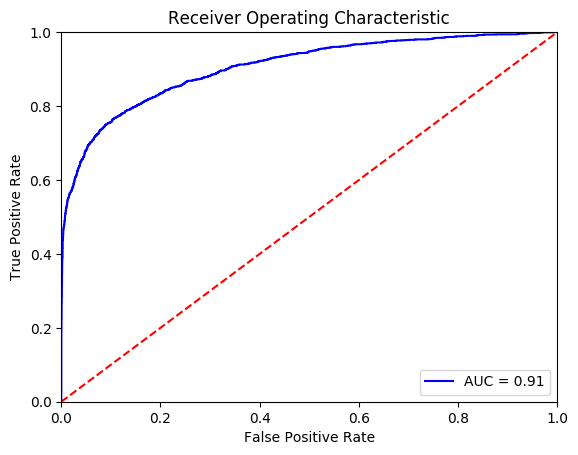
\includegraphics[width=0.6\linewidth]{AUC.png} \caption{ROC - AUC}
       \label{figure: AUC}    
  \end{figure}



Η μετρική Area Under the Curve(AUC) υπολογίζεται από το εμβαδόν που βρίσκεται κάτω από την καμπύλη ROC και τους άξονες και παίρνει τιμές στο [0,1]. Η μετρική AUC αποτελεί ένα μέτρο της διαχωρισιμότητας μεταξύ των κλάσεων. Η σημασία της θα γίνει καλύτερα αντιληπτή μέσω της εικόνας \ref{figure:aucExample} \cite{ROC}. Έστω ότι το σύνολο των πράσινων και κόκκινων κουκίδων αποτελεί το σύνολο ελέγχου. Οι κόκκινες κουκίδες παριστάνουν δείγματα της κλάσεις no rDR ενώ οι πράσινες ανήκουν στην κλάση rDR.
Ο άξονας κάτω από τις κουκίδες αναπαριστά την πρόβλεψη του μοντέλου για κάθε δείγμα.  

Αν τεθεί ως τιμή  κατωφλίου η τιμή του άξονα πριν το σημείο εμφάνισης του πρώτου πρασίνου(από αριστερά προς τα δεξιά), θα ταξινομηθούν λανθασμένα τέσσερα κόκκινα δείγματα της κλάσης no rDR στη κλάση rDR. Αν τεθεί ως τιμή κατωφλίου η τιμή του άξονα πριν το σημείο εμφάνισης του επόμενου δείγματος, τα δείγματα που θα ταξινομηθούν λάθος, θα είναι πέντε (ένα πράσινο και τέσσερα κόκκινα). Με την ίδια λογική μετατοπίζοντας το κατώφλι πριν το επόμενο δείγμα, θα συμβούν τέσσερις λάθος ταξινομήσεις (τρία κόκκινα και ένα πράσινο). Όπως είναι φανερό, με κανένα κατώφλι δεν δύναται να επιτευχθεί σωστή ταξινόμηση όλων των δειγμάτων του συνόλου ελέγχου, δηλαδή τέλειο διαχωρισμό κλάσεων και AUC =1. Μετά την παραπάνω ανάλυση μπορεί να γίνει εύκολα κατανοητό ότι η μετρική AUC αναπαριστά την πιθανότητα μία οποιαδήποτε εικόνα με rDR(πράσινες κουκίδες) να βρίσκεται στα δεξιά, μιας οποιασδήποτε εικόνας χωρίς rDR(κόκκινες κουκίδες) στον άξονα με τις προβλέψεις. 

\begin{figure}[!h]
    \centering
      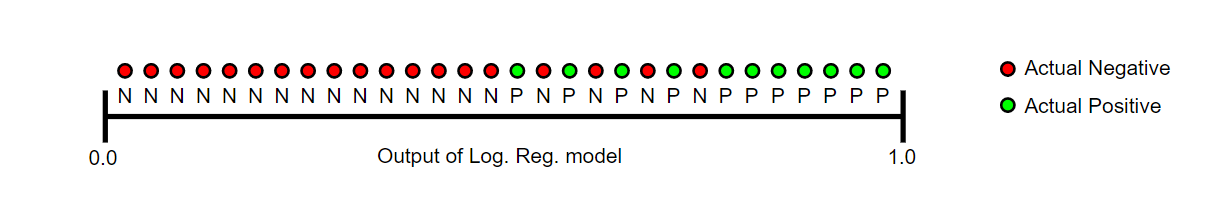
\includegraphics[width=1\linewidth]{auc_example.PNG} \caption{Αναπαράσταση προβλέψεων για ενα σύνολο δεδομενων πάνω σε άξονα}
       \label{figure:aucExample}    
  \end{figure}
  
  
  
\section{Υπολογισμός σημείων}
\label{sec:6.3}


\subsection{Σημείο υψηλής Ευαισθησίας}
\label{subsec:6.3.1}




Για να βρεθεί το σημείο υψηλής Ευαισθησίας(High Sensitivity), ορίζεται η μικρότερη αποδεκτή τιμή  Ευαισθησίας που ικανοποιεί τη συνθήκη για υψηλή Ευαισθησία. Έστω ότι μία εφαρμογή απαιτεί Ευαισθησία τουλάχιστον 0.9, για τιμές 0.9 και άνω, υπολογίζεται το άθροισμα (Ευαισθησία  + Εξειδίκευση) για τα διάφορα κατώφλια(thresholds). Σημείο υψηλής Ευαισθησίας ορίζεται το σημείο που μεγιστοποιεί το άθροισμα και περιγράφεται από την τριπλέτα [Sensitivity, Specificity, thresholds]. Στην \ref{eq:6new} παρουσιάζεται η μαθηματική περιγραφή για την εύρεση σημείου υψηλής Ευαισθησίας. 




\begin{equation} \label{eq:6new}
maximaze(Sens_{t} + Spec_{t}),~ για~ Sens_{t}>Sens_{min}
\end{equation}

όπου τα $Sens_{t}$ και $Spec_{t}$ αποτελούν τις τιμές Ευαισθησίας και Εξειδίκευσης αντίστοιχα σε ένα κατώφλι $t$ και η $Sens_{min}$ την ελάχιστη αποδεκτή τιμή της Ευαισθησίας.


\subsection{Σημείο υψηλής Εξειδίκευσης}
\label{subsec:6.3.2}
Η ίδια διαδικασία με την εύρεση σημείου υψηλής Ευαισθησίας ακολουθείται και για την εύρεση σημείου υψηλής Εξειδίκευσης οπότε παραλείπεται η περεταίρω ανάλυση. Στην \ref{eq:6bnew} παρουσιάζεται η μαθηματική περιγραφή για την εύρεση σημείου υψηλής Εξειδίκευσης. 


\begin{equation} \label{eq:6bnew}
maximaze(Sens_{t} + Spec_{t}),~ για~ Spec_{t}>Spec_{min}
\end{equation}

όπου τα $Sens_{t}$ και $Spec_{t}$ αποτελούν τις τιμές Ευαισθησίας και Εξειδίκευσης αντίστοιχα σε ένα κατώφλι $t$ και η $Spec_{min}$ την ελάχιστη αποδεκτή τιμή της Εξειδίκευσης.



\subsection{Βέλτιστο σημείο}
\label{subsec:6.3.3}
Ως βέλτιστο σημείο ορίζεται το σημείο στο οποίο μεγιστοποιείται το άθροισμα (Ευαισθησία + Εξειδίκευση). Καθώς το μοντέλο εκπαιδεύτηκε δίνοντας ίδιο βάρος στις δύο κλάσεις, το σημείο θεωρητικά παρουσιάζει σχετικά καλές τιμές στην πρόβλεψη και τον 2 κλάσεων(rdr/no rdr). Στην \ref{eq:6c} παρουσιάζεται η μαθηματική περιγραφή για την εύρεση βέλτιστου σημείου.


\begin{equation} \label{eq:6c}
maximaze(Sens_{t} + Spec_{t})
\end{equation}


  


